\documentclass[11pt]{article}
\usepackage[utf8]{inputenc}
\usepackage[T1]{fontenc}
\usepackage{graphicx}
\usepackage{grffile}
\usepackage{longtable}
\usepackage{wrapfig}
\usepackage{rotating}
\usepackage[normalem]{ulem}
\usepackage{amsmath}
\usepackage{textcomp}
\usepackage{amssymb}
\usepackage{capt-of}
\usepackage{hyperref}
\usepackage[margin=3cm]{geometry}
\usepackage{xfrac}
\usepackage{fancyhdr}
\usepackage{subfigure}
\usepackage{caption}
\usepackage{lipsum}
\usepackage{listings}
\usepackage{xcolor} % for setting colors
\usepackage{placeins} % put this in your pre-amble
\usepackage{flafter}  % put this in your pre-amble
\usepackage{rotating}

\usepackage[export]{adjustbox}
\title{Third deliverable}
\date{April 2018}
\author{Par4113: Jordi Bosch, Dean Zhu}

\begin{document}
\maketitle

\tableofcontents
\newpage

\section{Introduction}
The aim of these deliverable is to describe the perfect parallelism found when computing independent data. In our case the object to be studied is the mandelbrot set.

The mandelbrot set is formed by those complex numbers \emph{c} which do not diverge under the recurrence relationship: \[ z_0 = 0, z_{n+1}=(z_n)^{2} + c \]
It can be immediately seen that the verification whether each point belongs to our set is independent to each other as it only depends on the complex number chosen.

Points which belong to the set after k iterations are colored in white, other regions are colored according to the number of iterations before exiting the bounded region.

We are going to analyze how does the performance of the mandelbrot set calcuation behaves under several parallelization strategies and what causes some common pitfalls of these strategies.

Note that several metrics such as time elapsed are located in the corresponding directories.
\section{Tareador}

Before trying to apply parallelism to our code, we should first check what type of dependencies exists in order to be able to parallelize it correctly. We are going to consider two scenarios. First when we use a parallel strategy for the outer loop in our main function, hence parallelizing each row computation. And a second one where we parallelize each inner iteration.
\subsection{Row Granularity}
\begin{figure}[!htb]
  \includegraphics[max size={\textwidth}{0.7\textheight}]{./TareadorRow/row_mandel_dependency.png}
  \caption{Dependency graph of mandel.c, 8x8 image with row granularity}
\end{figure}
\begin{figure}[!htb]
  \includegraphics[max size={\textwidth}{0.7\textheight},angle=90]{./TareadorRow/row_mandeld_dependency.png}
  \caption{Dependency graph of graphic version of mandel.c, 8x8 image with row granularity, rotated 90 degrees}
\end{figure}
\FloatBarrier
Firstly we can see that both task dependency graph contain 8 different sized tasks. The reason for the discrepancy in size is caused by the way we compute which points belong to the mandelbrot set. As we run a while loop when a point is still in the convergence radius it makes the rows which contain more points belonging to the set run more iterations. As we are dividing it by rows it is logical that those closer to the origin have more points in the set and hence run more iterations to compute as they do not diverge.
The main difference we observe between the two graphs is the way the dependency edges are created. The graphical version of the program creates a sequential task dependency graph whereas the other version creates tasks which are totally independent from each other. After checking the code we can conclude that main culprit are these two lines:
\begin{verbatim}
XSetForeground (display, gc, color);
XDrawPoint (display, win, gc, col, row);
\end{verbatim}
It appears that the way it renders the final image is pixel by pixel in left to right and top to bottom order and hence it makes all pixel computations dependant on all previous tasks. If we comment out any one of those out both lines we can see that it behaves just as the non-graphic version, and if we only comment out one of them nothing changes.

\subsection{Point Granularity}
Just as the row granularity we observe the same patterns when using point granularity. The observation on parallelism and secuential execution still stands and moreover we get a further proof that points which seem to belong to the mandelbrot set take more iterations. Those are the tasks which take longer time.
\begin{figure}[!htb]
  \includegraphics[max size={\textwidth}{0.7\textheight}]{./TareadorPoint/point_mandel_dependency.png}
  \caption{Dependency graph of mandel.c, 8x8 image with point granularity}
\end{figure}
\begin{figure}[!htb]
  \includegraphics[max size={\textwidth}{0.7\textheight}, angle=90]{./TareadorPoint/point_mandeld_dependency.png}
  \caption{Dependency graph of graphic version of mandel.c, 8x8 image with point granularity, rotated 90 degrees}
\end{figure}
\FloatBarrier
\subsection{Parallelization strategy for Mandeld}
\label{sec:org733af78}
To avoid the sequential execution we want to be able to parallelize the process of drawing on the display. If we use tareador to check the task dependency we can observe that the global variable causing this problem is \emph{X11\_COLOR\_fake} which is used by both lines of code above. Hence we have to come up with a strategy so this variable can be used by all threads at once. Therefore one possible strategy is to create a critical region so there is no datasharing problem. If we use \texttt{tareador\_disable\_object(\&X11\_COLOR\_fake);} and create the corresponding dependency graph with tareador we can see it is now parallel.

\section{OpenMP Parallelization}

We are now going to try and parallelize the program with the above observations. There are various ways we can try to make the program parallel.

\subsection{Task directive}
First we are going to use the \texttt{task} directive to parallelize the program.

The directives to be added in to have row granularity and point granularity are respectively:
\begin{verbatim}
#pragma omp parallel
#pragma omp single
    for (row = 0; row < height; ++row) {
#pragma omp task firstprivate(row, col)
        for (col = 0; col < width; ++col) {
...
\end{verbatim}
\begin{verbatim}
#pragma omp parallel
#pragma omp single
    for (row = 0; row < height; ++row) {
        for (col = 0; col < width; ++col) {
#pragma omp task firstprivate(row, col)
            { 
...
\end{verbatim}
\begin{figure}[!htb]
  \begin{minipage}[t]{0.48\textwidth}
    \centerline{\includegraphics[width=1.5\linewidth]{./Task/row/row.pdf}}
    \caption{Task directive with row granularity}
  \end{minipage}
  \begin{minipage}[t]{0.48\textwidth}
    \centerline{\includegraphics[width=1.5\linewidth]{./Task/point/point.pdf}}
    \caption{Task directive with point granularity}
  \end{minipage}
\end{figure}

We can see that the row based granularity has a strong parallelism, as the speedup grows linearly with the increase of threads. This seems to line up with the hypothesis that the Mandelbrot Set computation is perfectly parallelizable. However we do see an unexpected result when using the point granularity, It seems that due to the number of tasks created, the overhead created to synchronize and fork is too large for it to be worth parallelizing.

\FloatBarrier
\subsection{Taskloop directive}
Another possible strategy is using the \texttt{taskloop} directive.  

In this cases our final code for row and point granularity should look like this:

\begin{verbatim}
#pragma omp parallel
#pragma omp single
#pragma omp taskloop num_tasks(width/8) private(col)
    for (row = 0; row < height; ++row) {
...
\end{verbatim}
\begin{verbatim}
#pragma omp parallel
#pragma omp single
    for (row = 0; row < height; ++row) {
#pragma omp taskloop num_tasks(width/8) firstprivate(row)
        for (col = 0; col < width; ++col) {
...
\end{verbatim}

\begin{figure}[!htb]
  \begin{minipage}[t]{0.48\textwidth}
    \centerline{\includegraphics[width=1.5\linewidth]{./Taskloop/row/row.pdf}}
    \caption{Taskloop directive with row granularity}
  \end{minipage}
  \begin{minipage}[t]{0.48\textwidth}
    \centerline{\includegraphics[width=1.5\linewidth]{./Taskloop/point/point.pdf}}
    \caption{Taskloop directive with row granularity}
  \end{minipage}
\end{figure}
\FloatBarrier
Our first decision in this optimization was to choose the grainsize or the number of tasks. We opted for creating width/64 number of tasks. This meant that the computation space was divided in enough chunks so we could have enough load balancing but not too much to avoid excessive overhead. 
Similar to the last case we can see that using the taskloop with a row granularity possesses the characteristics of strong parallelism. Even though there should be a better grainsize to further optimize the execution, the same holds true for the point parallelism now as the grainsize is larger.

\subsection{For directive}

When using the \texttt{for} directive we have a few choices to make. First of all, it is necessary to choose a scheduling strategy, in addition it is also recommendable to choose a chunk size, also due to the fact that the points are independent to one and other we can and should add a nowait clause to properly run a parallel process. 

\begin{figure}[!htb]
  \begin{minipage}[t]{0.48\textwidth}
    \centerline{\includegraphics[width=1.5\linewidth]{./For/row/row.pdf}}
    \caption{Comparison of different schedulings with row granularity}
  \end{minipage}
  \begin{minipage}[t]{0.48\textwidth}
    \centerline{\includegraphics[width=1.5\linewidth]{./For/point/point.pdf}}
    \caption{Comparison of different schedulings with point granularity}
  \end{minipage}
\end{figure}
\FloatBarrier
We compare the speedup and time taken for 5 different strategies. We see that when we consider the row granularity, the slowest one is indeed the sequential execution. What might be surprising at first sight is the time taken for the static directive without specifying chunk size. 

If we analyze the code, we observe that the computational cost of the program is mostly on the while loop inside the main function. We can see that the time taken for each point can range from 1 to the maximum number of iterations. That means that although the program is perfectly parallelizable not all the points take the same time, that is, this is an unbalanced problem.

Returning to our first point, now it seems obvious that the reason for the elapsed time in the static scheduling is caused by load unbalance, as by default it uses chunks of size \(\frac{Problem Size}{Num threads}\). 

The other three strategies seem to have similar runtimes, with static and dynamic being slightly more effecient than guided. The most probable reason for guided to be slower is that it uses quite large tasks at the beginning, so it is then possible that we have a task unbalance caused by the first few tasks which causes a slight overhead in contrast to the other two faster parallelizations. 

Now, in our second case when using the \texttt{for} directive with point granularity, we can see that the problem with load balancing still exists but it is fixed for guided, in fact it is faster than the other two. The problem which we mentioned above ceases to exist as we have a quadratic amount of iterations due to being a finer granularity.\\

We can assert our hypothesis by checking the statistics provided with \texttt{Paraver}

\begin{center}
  \begin{tabular}{|l|l|l|l|l|}
    \hline
    & static & static,10 & dynamic,10 & guided,10\\
    \hline
    Running average time per thread (ns) & 444744267  & 460634932  & 483308567 & 463425925\\
    \hline
    Execution unbalance & 0.32325 & 0.68096 & 0.64334 & 0.38661 \\
    \hline
    SchedForkJoin (ns) & 986174371 & 36243060 & 25199996 & 509464058 \\
    \hline
  \end{tabular}
\end{center}

Indeed, we see that there is a big discrepancy in the execution unbalance. While the average running time is similar, we can see that the ratio between average time and maximum time is doubled when using static and guided instead of static with smaller chunks or dynamic. This also causes large joining overhead as many threads have to wait before being able to finish. As guided divides tasks better at later iteration, then it is also logical that its synchronization average is lower than the one of static which causes their difference in elapsed time.


\begin{figure}[!htb]
  \centerline{\includegraphics[width=0.9\linewidth]{./For/Paraver/static.png}}
  \caption{Paraver statistics for static scheduling}
\end{figure}
\begin{figure}[!htb]
  \centerline{\includegraphics[width=0.9\linewidth]{./For/Paraver/static10.png}}
    \caption{Paraver statistics for static,10 scheduling}
\end{figure}
\begin{figure}[!htb]
  \centerline{\includegraphics[width=0.9\linewidth]{./For/Paraver/dynamic.png}}
    \caption{Paraver statistics for dynamic,10 scheduling}
\end{figure}
\begin{figure}[!htb]
  \centerline{\includegraphics[width=0.9\linewidth]{./For/Paraver/guided.png}}
    \caption{Paraver statistics for guided,10 scheduling}
\end{figure}

\FloatBarrier
\subsection{For directive with Collapse}
When we use the \texttt{collapse(2)} directive, we are assuming that the two for loops are correctly nested and we are running through a \(N*M\) computational space and we will let each thread compute a rectangular space. Hence if we try and compute this we will see a similar behaviour to the \texttt{for} directive with row granularity as the division is not as fine as point granularity.

\begin{figure}[!htb]
  \centerline{\includegraphics[width=0.9\linewidth]{./For/Collapse/collapse.pdf}}
\end{figure}

\subsection{For directive with task creation}
In this new strategy our aim is to create tasks parallelly to reduce its overhead. And indeed if we check the speedup of this strategy it increases all strategies to almost a 7x speedup. That is, compared to the \texttt{for} directive we don't have the problem of load unbalancing as we are only using it to create tasks. And also we do not have the problem of excessive overhead obtained from creating \(N*N\) tasks as we have them evenly divided.

\begin{figure}[!htb]
  \centerline{\includegraphics[width=0.9\linewidth]{./For/ForTask/fortask.pdf}}
\end{figure}

\section{Conclusion}
After analyzing the process of calculation of the mandelbrot set we have discovered several characteristics. \\
Its calculation is an embarrassingly parallel problem while also being unbalanced. To properly parallelize this problem we have two main steps. First we should divide the workload to several threads and later on compute all the work on each thread. \\
This means that while the problem is perfectly parallelizable not every strategy tackles the problem correctly and there are other factors to take into consideration, in our case the biggest culprits are load unbalance and fork/synchronization oberhead.
Due to the reasons we mentioned we encounter several problems. If we divide into tasks thoughtlessly we might cause a load unbalance (static scheduling). But if we want to avoid load unbalance and use really fine partitions of the problem we might run into a gigantic overhead caused by the creation of tasks (task directive with point granularity, and in a lesser extent taskloop directive with point granularity). All other strategies seem to deal more or less well with this problem, which is to be expected as it is perfectly parallelizable, as a result we see that most strategies have a strong scalability.


\end{document}